\documentclass[landscape, a0]{sciposter}
% Hentet fra http://iacs.epfl.ch/colloqnum06/poster.html
\usepackage[utf8]{inputenc}
\usepackage[T1]{fontenc}
\usepackage[english]{babel}

\usepackage{amsmath}
\usepackage{amssymb}
\usepackage{multicol}
\usepackage{graphicx}
\usepackage{listings}

\usepackage{epstopdf}
\usepackage{mwe}% for example images

\newcommand{\subcaption}[1]% %1 = text
{\refstepcounter{subfig}%
\par\vskip\abovecaptionskip
\centerline{\textbf{(\alph{subfig})} #1}%
\vskip\belowcaptionskip\par}

% create subfigure environment
\def\subfigure{\let\oldcaption=\caption
\let\caption=\subcaption
\minipage}
\def\endsubfigure{\endminipage
\let\caption=\oldcaption}

\usepackage{xcolor}

\definecolor{dkgreen}{rgb}{0,0.45,0}
\definecolor{gray}{rgb}{0.5,0.5,0.5}
\definecolor{mauve}{rgb}{0.30,0,0.30}

\lstset{frame=tb,
	language=Python,
	aboveskip=4mm,
	belowskip=5mm,
	showstringspaces=false,
	columns=flexible,
	basicstyle={\small\ttfamily},
	numbers=left,
	numberstyle=\footnotesize,
	keywordstyle=\color{dkgreen}\bfseries,
	commentstyle=\color{dkgreen},
	stringstyle=\color{mauve},
	frame=single,
	breaklines=false,
	breakatwhitespace=false,
	tabsize=4,
}


\usepackage{pgfplots}
\pgfplotsset{
	compat=1.5,
    box plot/.style={
        /pgfplots/.cd,
        black,
        only marks,
        mark=-,
        mark size=1em,
        /pgfplots/error bars/.cd,
        y dir=plus,
        y explicit,
    },
    box plot box/.style={
        /pgfplots/error bars/draw error bar/.code 2 args={%
            \draw  ##1 -- ++(1em,0pt) |- ##2 -- ++(-1em,0pt) |- ##1 -- cycle;
        },
        /pgfplots/table/.cd,
        y index=2,
        y error expr={\thisrowno{3}-\thisrowno{2}},
        /pgfplots/box plot
    },
    box plot top whisker/.style={
        /pgfplots/error bars/draw error bar/.code 2 args={%
            \pgfkeysgetvalue{/pgfplots/error bars/error mark}%
            {\pgfplotserrorbarsmark}%
            \pgfkeysgetvalue{/pgfplots/error bars/error mark options}%
            {\pgfplotserrorbarsmarkopts}%
            \path ##1 -- ##2;
        },
        /pgfplots/table/.cd,
        y index=4,
        y error expr={\thisrowno{2}-\thisrowno{4}},
        /pgfplots/box plot
    },
    box plot bottom whisker/.style={
        /pgfplots/error bars/draw error bar/.code 2 args={%
            \pgfkeysgetvalue{/pgfplots/error bars/error mark}%
            {\pgfplotserrorbarsmark}%
            \pgfkeysgetvalue{/pgfplots/error bars/error mark options}%
            {\pgfplotserrorbarsmarkopts}%
            \path ##1 -- ##2;
        },
        /pgfplots/table/.cd,
        y index=5,
        y error expr={\thisrowno{3}-\thisrowno{5}},
        /pgfplots/box plot
    },
    box plot median/.style={
        /pgfplots/box plot
    }
}


% =========================================================
% ====== Farver og grafik øverst på siden =================
% =========================================================
% Definer farven på baggrunden i overskrifts boksene
\definecolor{BoxCol}{rgb}{0.9,0.9,1}

% Definer farven på tekstn i overskrifts boksene
\definecolor{SectionCol}{rgb}{0,0,0}

% Indsæt logo / billede ved siden af titlen på posteren
\leftlogo[1.6]{fig/julia} 
\rightlogo[1.1]{fig/sdu_segl.pdf} 

% Sæt bredden af de vertikale linier mellem spalterne
\setlength{\columnseprule}{1pt}

% Sæt afstanden mellem to kolonner
%\setlength{\columnsep}{20pt}

% =========================================================
% ====== Informationer om hvem der står bag posteren ======
% =========================================================
% Definer informationer omkring titel, forfattere og 
% organisationen bag.
\title{Who's Julia?}

% Note: only give author names, not institute
\author{Simon Knudsen, Sonni Jensen, Asbjørn Jensen}
 
% insert correct institute name
\institute{Department of Mathematics and Computer Science,\\
	University of Southern Denmark\\}

%define conference poster is presented at (appears as footer)
\conference{FF501 poster session, Juni 2016 SDU Odense}


% =========================================================
% ====== Start på selve indholdet af posteren =============
% =========================================================
\begin{document}

\maketitle

%%% Begin of Multicols-Enviroment
\begin{multicols}{3}


% =========================================================
% ====== Første del =======================================
% =========================================================
\section{Julia}
Julia is an object-oriented programming language, which has been under development since 2009. First released in 2012 and the newest stable version of Julia is version 0.4.5. The language has been created because the developers wanted a language with all the features they like from other languages. \\
\\
The developers wanted the language to be open source, which means that everybody can read and modify the language. One of the ideas was to make the language as simple, readable and easy to learn as possible. The language is made for high performance and scientific computations while still supporting general purpose programming.
% =========================================================
% ====== Anden del ========================================
% =========================================================
\section{Goal}
The goal of this project is to benchmark Julia and do speed comparison with Python, C++ and Java. The run time is measured as CPU time with the terminal command \textbf{time} and built-in profiling tools in the given language.
\section{Syntax}
\begin{multicols}{3}
	\begin{figure}[H]
\begin{lstlisting}[frame=none, numbers=none]
a = 0

for i = 1 : 10
	a += i
end

while a > 2
	i -= 1
end

function hello(name)
	println("Hello $name")
end 
hello("Julia") 
\end{lstlisting}
	\end{figure}
	\hfill
	\begin{figure}[H]
\begin{lstlisting}[frame=none, numbers=none]
b = 20

for i = 10 : -1 : 1
	b -= 1
end

if a < b
	println(b / a)
elseif a > b
	println(a / b)
else
	println(a + b)
end
		\end{lstlisting}
	\end{figure}
	\hfill
	\begin{figure}[H]
\begin{lstlisting}[frame=none, numbers=none]
array = fill(1, 100)

for i = 2 : 100
	array[i] += array[i-1]
end

for i in array
	println(i)
end

minimum(array)
maximum(array)
sum(array)
		\end{lstlisting}
	\end{figure}
\end{multicols}
\section{Project Euler problem 116}
\textit{A row of five black square tiles is to have a number of its tiles replaced with coloured tiles from red(length two), green(length three), or blue(length four). If red tiles are chosen there are seven ways. If green tiles are chosen there are three ways. And if blue tiles are chosen there are two ways. Assuming that colours cannot be mixed there are $7+3+2=12$ ways of replacing the black tiles in a row measuring five units in length.}
\hspace*{-1in}
\begin{figure}[H]
	\centering
	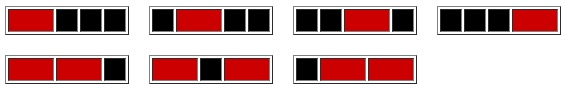
\includegraphics[scale=1.635]{fig/1161.jpg}
	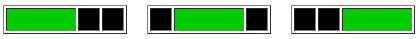
\includegraphics[scale=2.2]{fig/1162.jpg} 
	
\includegraphics[scale=2.2]{fig/1163.jpg} 
\end{figure}
\hspace*{-0.3in}
\begin{figure}[H]
	\centering
	\begin{lstlisting}
	function solve(tileSize, length)
		if tileSize > length
			return 0
		end
		solutions = 0
	
		for i = tileSize : length
			solutions += 1
			solutions += solve(tileSize, length-i)
		end
	
		return solutions
	end
	
	function calc(size)
		result = solve(2, size) #Red tiles
		result += solve(3, size) #Green tiles
		result += solve(4, size) #Blue tiles
	
		return result
	end
	\end{lstlisting}
	\caption{Julia implementation}
\end{figure}

\vspace*{-1.4in}
\begin{figure}
 \centering
 \hspace*{-2.5in}
 \begin{subfigure}{0.30\textwidth}
		\centering
		\scalebox{1.4}{
		\begin{tikzpicture}
			\begin{axis} [
			title=Julia,
			xlabel={$length$},
			ylabel={$seconds$},
			grid=major,]
				\addplot [box plot median] table {../graphdata/euler116ub-julia-box.dat};
				\addplot [box plot box] table {../graphdata/euler116ub-julia-box.dat};
				\addplot [box plot top whisker] table {../graphdata/euler116ub-julia-box.dat};
				\addplot [box plot bottom whisker] table {../graphdata/euler116ub-julia-box.dat};
				\addplot table {../graphdata/euler116ub-julia.dat};
			\end{axis}
		\end{tikzpicture}
		}
 \end{subfigure}
 \hspace*{2in}
 \begin{subfigure}{0.30\textwidth}
		\centering
		\scalebox{1.4}{
		\begin{tikzpicture}
			\begin{axis} [
			title=Python,
			xlabel={$length$},
			grid=major,]
				\addplot [box plot median] table {../graphdata/euler116ub-python-box.dat};
				\addplot [box plot box] table {../graphdata/euler116ub-python-box.dat};
				\addplot [box plot top whisker] table {../graphdata/euler116ub-python-box.dat};
				\addplot [box plot bottom whisker] table {../graphdata/euler116ub-python-box.dat};
				\addplot table {../graphdata/euler116ub-python.dat};
			\end{axis}
		\end{tikzpicture}
		}
 \end{subfigure}
 
 \hspace*{-2.18in}
 \begin{subfigure}{0.30\textwidth}
		\centering
		\scalebox{1.4}{
		\begin{tikzpicture}
			\begin{axis} [
			title=Java,
			xlabel={$length$},
			ylabel={$seconds$},
			grid=major,]
				\addplot [box plot median] table {../graphdata/euler116ub-java-box.dat};
				\addplot [box plot box] table {../graphdata/euler116ub-java-box.dat};
				\addplot [box plot top whisker] table {../graphdata/euler116ub-java-box.dat};
				\addplot [box plot bottom whisker] table {../graphdata/euler116ub-java-box.dat};
				\addplot table {../graphdata/euler116ub-java.dat};
			\end{axis}
		\end{tikzpicture}
		}
 \end{subfigure}%
 \hspace*{1.73in}
 \begin{subfigure}{0.30\textwidth}
		\centering
		\scalebox{1.4}{
		\begin{tikzpicture}
			\begin{axis} [
			title=C++,
			xlabel={$length$},
			grid=major,]
				\addplot [box plot median] table {../graphdata/euler116ub-cpp-box.dat};
				\addplot [box plot box] table {../graphdata/euler116ub-cpp-box.dat};
				\addplot [box plot top whisker] table {../graphdata/euler116ub-cpp-box.dat};
				\addplot [box plot bottom whisker] table {../graphdata/euler116ub-cpp-box.dat};
				\addplot table {../graphdata/euler116ub-cpp.dat};
			\end{axis}
		\end{tikzpicture}
		}
 \end{subfigure}
 
 \hspace*{-7.00cm}
 \begin{subfigure}{0.30\textwidth}
		\centering
		\scalebox{1.4}{
		\begin{tikzpicture}
			\begin{axis} [
			title=Comparison,
			xlabel={$length$},
			ylabel={$seconds$},
			grid=major,
			]
			\addplot table {../graphdata/euler116ub-julia.dat};
			\addplot table {../graphdata/euler116ub-java.dat};
			\addplot table {../graphdata/euler116ub-cpp.dat};
			\addplot table {../graphdata/euler116ub-python.dat};
			\end{axis}
		\end{tikzpicture}
		}
 \end{subfigure}
 \hspace*{4.5cm}
 \begin{subfigure}{0.30\textwidth}
		\centering
		\scalebox{1.4}{
			\begin{tikzpicture}
			\begin{axis} [
			title=Comparison - Python excluded,
			xlabel={$length$},
			grid=major,
			legend entries={$Julia$,$Java$,$c++$,$Python$},
			legend style={at={(1,1)},anchor=north west},
			]
			\addplot table {../graphdata/euler116ub-julia.dat};
			\addplot table {../graphdata/euler116ub-java.dat};
			\addplot table {../graphdata/euler116ub-cpp.dat};
			\end{axis}
			\end{tikzpicture}
	}
 \end{subfigure}
 %\caption{fig}
\end{figure}

% =========================================================
% ====== Afsnit ===========================================
% =========================================================
\subsection{Results of Project Euler 116}
It is clear that the graphs are exponential increasing. Another thing to notice is that the input is only increasing by one but is still making a huge difference in the run time. One of the reasons is that the problem is solved with recursion, for every extra one bit of space added to the black box a lot more recursive calls will have to be made.\\
\\
The difference in time between the four languages are as expected. Python does not support any form of tail recursion optimization and the result is really slow. Java and Julia on the other hand does a good job at optimizing the recursive calls and is actually faster than C++ - keep in mind that no compiler flags were used in C++, so the default optimization level is used.\\
\\
Julia and Java is close but Java is a bit faster, which is expected because of the fact that Java has been in development much longer than Julia and has a lot more optimization than Julia.

\section{Pros and Cons of Julia}
\textbf{Advantages:}
\begin{list}{}{}
	\item[$\bullet$] Julia is easy to learn and software are easily made.
	\item[$\bullet$] Julia does good compiler optimizations, which sometimes makes Julia as fast as C++.
	\item[$\bullet$] In overall test Julia performed very well.
	\item[$\bullet$] Julia was the only language that did not cause any out of memory issue at some point.
\end{list}
\textbf{Disadvantages:}
\begin{list}{}{}
	\item[$\bullet$] Compiler optimization can break (Dual pivot quicksort)
	\item[$\bullet$] Julia is not very flexible.
	\item[$\bullet$] Missing features and weird behaviors with implementing code from other languages.
\end{list}

\section{Conclusion}
It can be difficult to make any conclusions by the benchmarking but it may give an idea of how Julia performs, compared to Java, Python and C++. One thing to keep in mind is that Julia is in version 0.4.5 - it has yet to reach version 1.0.0. This could mean that Julia might get even faster in the future and by the benchmarking it does look as Julia is already performing well. \\ \\ The developers are trying to make a programming language that is as easy to learn and write as Python but with a compiler that optimizes code like Java and both of these goals have more or less been reached already. Julia was definitely easy to learn and by the benchmarking it does look like that the compiler is doing well with the optimization. It also feels like the Julia developers are playing with the idea of giving the user some control over what is happening behind the scene. ‘Playing’ because this does not feel close to done. The user can allocate memory for a variable manually, but if a new value is assigned to the variable, the memory size is also changed. It is not possible to free a declared variables memory entirely and the only operation the user can do with the garbage collector is force garbage collection and disable the garbage collector. 

\begin{thebibliography}{m}

Julia's offical homepage\\
www.julialang.org\\
\\
Project Euler\\
www.projecteuler.net


\end{thebibliography}


\end{multicols}

\end{document}

